\documentclass[letterpaper,10pt]{article}
\usepackage{biblatex} %Imports biblatex package
\addbibresource{references.bib} %Import the bibliography file
\usepackage{graphicx} % Required for inserting images
\usepackage{float}

\title{What are effective pumping strategies to perform well on flats in slalom and what is a good training strategy to learn these strategies}
\author{Christian Magelssen}
\date{January 2024}

\begin{document}

\maketitle

\section{Background}

In alpine ski racing, the goal is to ski a slalom course in the shortest time possible. Descents can be executed in nearly any way, as long as the athlete passes on the correct side of the gates placed along the slope. This aspect introduces a significant degree of freedom in technique selection. To address this freedom of choice, researchers have sought to identify the strategies and techniques employed by athletes to tackle this challenge.

Understanding these strategies is crucial knowledge for coaches to enhance their training practices. It helps coaches identify which techniques and strategies may be beneficial to emphasize in training sessions. However, a key challenge in this research is the diverse nature of alpine skiing situations. Principles derived from one scenario may not necessarily apply to another. This highlights the need for a nuanced approach, recognizing that what works in one situation may not be universally applicable to others.



I alpint er målet å kjøre raskest mulig ned en løype på tid. Nedkjøringer kan gjøres på nesten alle mulige måter så lenge utøveren passerer på riktig side av porten som er plassert nedover bakken, og innbyr derfor til et stort frihetsgradsproblem. For å dette frihetsgradsproblemet har forskere forsøkt å finne ut hvilke strategier og teknikker utøvere bruker for å løse dette frihetsgradsproblemet. Dette er viktig kunnskap som trenere kan bruke i sin trenerpraksis, som å vite hvilke teknikker og strategier det kan være fornuftig å stimulere til i treningsarbeidet. En utfordring med dette arbeidet er at situasjonene i alpint er svært forskjellige, slik prinsipper fra en situasjonen ikke nødvendigvs gjelder en annen. Det betyr 


. Derfor har forskere forsøkt å studere hvilke mekanismer som er lagt til grunn for dette arbeidet. En utfordring med dette arbeidet er at situasjonene i alpint, som betyr at det vanskelig å studere noe i en situasjon. Derfor er det viktig å belyse teknikk, men det er like mye 

Det ekspert performance approach er en teoretisk tilnærming som omhandler hvordan gir et teoretisk rammeverk for å studere alpint. Rammeverket går ut på. Med utgangspunkt i dette teoretiske rammeverket har denne studien forsøkt å finne ut hva som er en. Vi fokuserer på tekniske ferdigheter.

\section{Introduction}


\subsection{What distinguishes skilled performers from less skilled performers?}

The first step in the expert performance approach is to capture differences that discriminate between the best and less skilled performers in alpine skiing. Then, to design representative tasks that allow experts to reproduce their superiority.

Alpine ski racers often compete with small time differentials in completing a slalom course. For instance, in a slalom race, the discrepancy between the victor and the second-place finisher might be as slight as a few hundredths of a second after two runs on a 50-second course. Despite the narrow margin in overall race time, the time gaps between skiers can be substantial when examining specific smaller segments of the slalom course. Three such crucial segments, identified through previous gate-to-gate analysis or shorter intermediate sections, are the course's hairpins, starts, and flat sections. These observations suggest that even the most skilled performers have room for improvement in particular parts of a course.

In my doctoral project, I chose to study the flat sections in a slalom course. The rationale for this choice was that the race hill in Oslo's new indoor ski hall consisted of a long, flat section that made it great for studying this skill. The skill is also more generic than the hairpin and the start since the flats in slalom typically cover a greater proportion of the course compared to the hairpin and the start. Moreover, an effective technique for skiing flats might also be generalized to hairpins. For these reasons, I studied the flat section in alpine ski racing. 


\subsection{How do skilled performers perform better?}
In this doctoral research project, I have chosen to study flat slopes in slalom skiing. The goal in the next phase of the expert performance approach is to identify causal mechanisms that can explain the superior performance of skilled performance in this section of the slalom course \cite{williams_using_2017}. 


The goal of the second phase of the expert performance approach is to understand mechanisms that explains the better performance in the skilled athlete. 

En tilnærming for å kjøre fortere på flater er å kjøre renere. En annen mer offensive strategi er å pumpe for å kjøre fortere på flater. I modellen til noen forskere ble. Et viktig poeng med modellen var dermed å. Et viktig element i studien var dermed å finne ut om.    

Yet, in an experiment conducted (unpublished data), our research group observed that elite skiers produced faster times in a free skiing course of gentle terrain when they made slalom turns using the pumping technique (that is, moving one’s centre of mass towards the centre of the turn) compared to straight gliding runs. This finding was an initial proof of concept that skiers could increase the velocity through muscular work by an amount larger than the potential energy was able to account for. Velocity gains exceeding the contribution of the gravitational force has also been reported in other studies4,6. For example, Reid noted that skiers sometimes achieved such effects in the transition between two slalom turns. Although there is data to support pumping as a skiing technique to increase velocity, no study has looked at the exact actions resulting in this effect. This is an important topic to study because the pumping technique has been a cornerstone in the Norwegian Ski Federation’s (NSF) technique strategy since the experiment on pumping was conducted eight years ago. Despite many efforts to improve this skill, our experience is that some skiers merit more from this technique than others but that it is difficult to pinpoint precisely what good and bad ‘pumpers’ are doing differently. Understanding the motion actions that underpin an effective pumping technique is, therefore, an important subject to study.

Owing to the importance of this skill for sporting performance for experienced and well-trained athletes, it is also critical to understand how we can optimise skill learning to enhance this skill. In experimental psychology and cognitive neuroscience, there is converging evidence showing that certain type of practices, as well as the distribution of it, contributes more effectively to the attainment of expertise than other types of practices7–10. If the effective learning paradigms discovered in this research is true, it could fundamentally alter the way coaches typically design practices for skill learning. However, as most of these studies have relied on simpler laboratory-based tasks using novices as participants5 the translation to a real-world complex sport, such as alpine ski racing and with very skilled athletes is not clear. 


\subsection{Why do skilled performers perform better?}
The final stage in the expert performance approach is to understand how.

\subsection{What is motor skill learning?}
Vi har ofte lite utfordring med å identifisere en god prestasjon når vi ser det. For eksempel kan vi si at en alpinist som kjører rene og raske svinger ned et bratt og isete heng i slalåm for å være skilled. Til tross for dette, klarer ikke forskere å enes om en bestemt definisjon hva det er. Noen forskere har heller forsøkt å snevre inn motor skill learning ved å eksludere hva det ikke er. Ved å gjøre det snakker man ofte om at skilled performance er å utføre en bevegelse snarere enn å kommunisere hva man kan fortelle om ferdigheten. Man skiller også motor skill learning fra adaptasjonsprosesser som ofte blir tilbakestilt med en gang. På et overordnet nivå dreier motorisk læring seg om å successfully achieve goals. Når dette er snakk om motorisk handlinger, snakker vi om motorisk utførelse.

Forskere har på en annen side begynt å lande på hvilke komponenter som inngår i ferdighetslæring. På den ene siden handler det om å velge gode strategier (action selection). For eksempel må en alpinist bestemme seg for om man skal velge en lang linje eller kort linje ned i fart. Når denne strategien er valgt er det viktig at denne handlingen utføres så presist og godt som mulig (action execution). Til slutt er det viktig at disse handlingene utføres så presist som mulig. 

Et kanskje tredje element er å velge gode strategier. Kanskje si noe om de læringmekanismene som støtter dette. 


- Multiple learning mechanism

\subsection{Deliberate practice}
Et viktig aspekt for å utvikle ekspertise er deliberate practice. Deliberate practice kan kjennetegnes ved at å forsøker å hele tiden. Selv om noen. For å få til deliberate practice er det nødvendig med en god oversikt over strategier 





\subsection{Designing practice to make skilled performers learn}



What can coaches do to train deliberate practice?






I den siste fasen forsøker man å finne ut hvordan eksperter tilegner seg ferdighetene for å kjøre for på flater. 


Deliberate practice and strategies

Adaptive and skilful

I





et viktig innsikt er at. et viktig innsikt ermed hvordan de presterer bedre. er de


- Tilrettelegging og veiledning


Organisation, Instruction and feedback


Contextual interference





Reinforcement learning





\subsection{Aims}




\section{Method}

\subsection{Sample and approach}


\section{Results}


\subsection{How do skilled performers perform better on flat section in slalom?}

I studie 3 definerte vi i tillegg tre andre strategier for å studere. Her har vi valgt å studere effektene av disse strategiene på flatekjøring i alpint. For å gjennomføre denne analysen har vi kun valgt å hente ut tidene fra forced exploration økten der vi har observasjoner fra alle deltakerne på alle strategiene. Vi fant at deltakerne i gjennomsnitt kjørte raskest med strekk og skyv, etterfølgt av b,c og a, som var i forvented rekkefølge. Vi fant at utøverne i snitt kjørte best med. Figur viser denne. 

Det som er interessant med denne analysen er at strekk ser ut til å være den soleklart viktigste mekanismen for å kjøre fort på flater blant denne populasjonen av utøvere. Isolert var også skyv en effektiv strategi, men så ikke ut til å bidra stort da den ble lagt til strekk. En forklaring på dette er at utøverne var langt. Det er likevel greit å merke seg at utøverne. Selm om det var en global trend til at strekk og skyv var best, var det også variasjoner i dette. 

I tillegg har vi sett på om.. Vi har derfor studert om det er en tillegssfordel ved å bruke andre strategier. I gjennomsnitt fant vi at 


\begin{figure}[H]
\centering
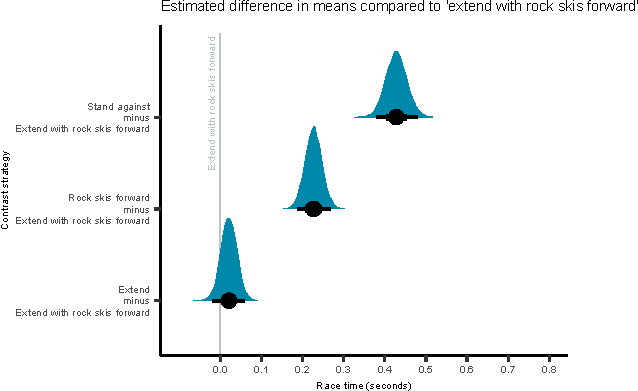
\includegraphics{figure_results_Q1_strategies.pdf}
\caption{Illustration of the experimental design and procedure. \textbf{a.} Timeline of the three-day learning experiment. During the baseline session, the skiers raced a slalom course in the shortest time possible without receiving race time feedback. The skiers were then assigned to three learning groups (see b). In their assigned group, the skiers underwent three acquisition sessions, comprising one forced exploration session (skiers performed all strategies) and two free choice sessions (skiers or coaches could choose strategies themselves). On the last day, skiers completed a retention and transfer test where they could pick strategy themselves, again without receiving race time feedback. \textbf{b.} Illustration of the learning groups in the study. The supervised (target skill) learning group involved coaches consistently choosing the theoretically best strategy (except during forced exploration), while the supervised (free choice) learning group allowed coaches to freely select strategies. The skiers in both of these learning groups received feedback on strategy execution from their assigned coach, while the skiers in the reinforcement learning group independently selected strategies and received feedback from the timing system to facilitate value learning of each strategy}
\label{fig:experiment}
\end{figure}



\section{Discussion}

\section{}

\printbibliography

\end{document}
